\begin{figure*}[t]
  \begin{center}
    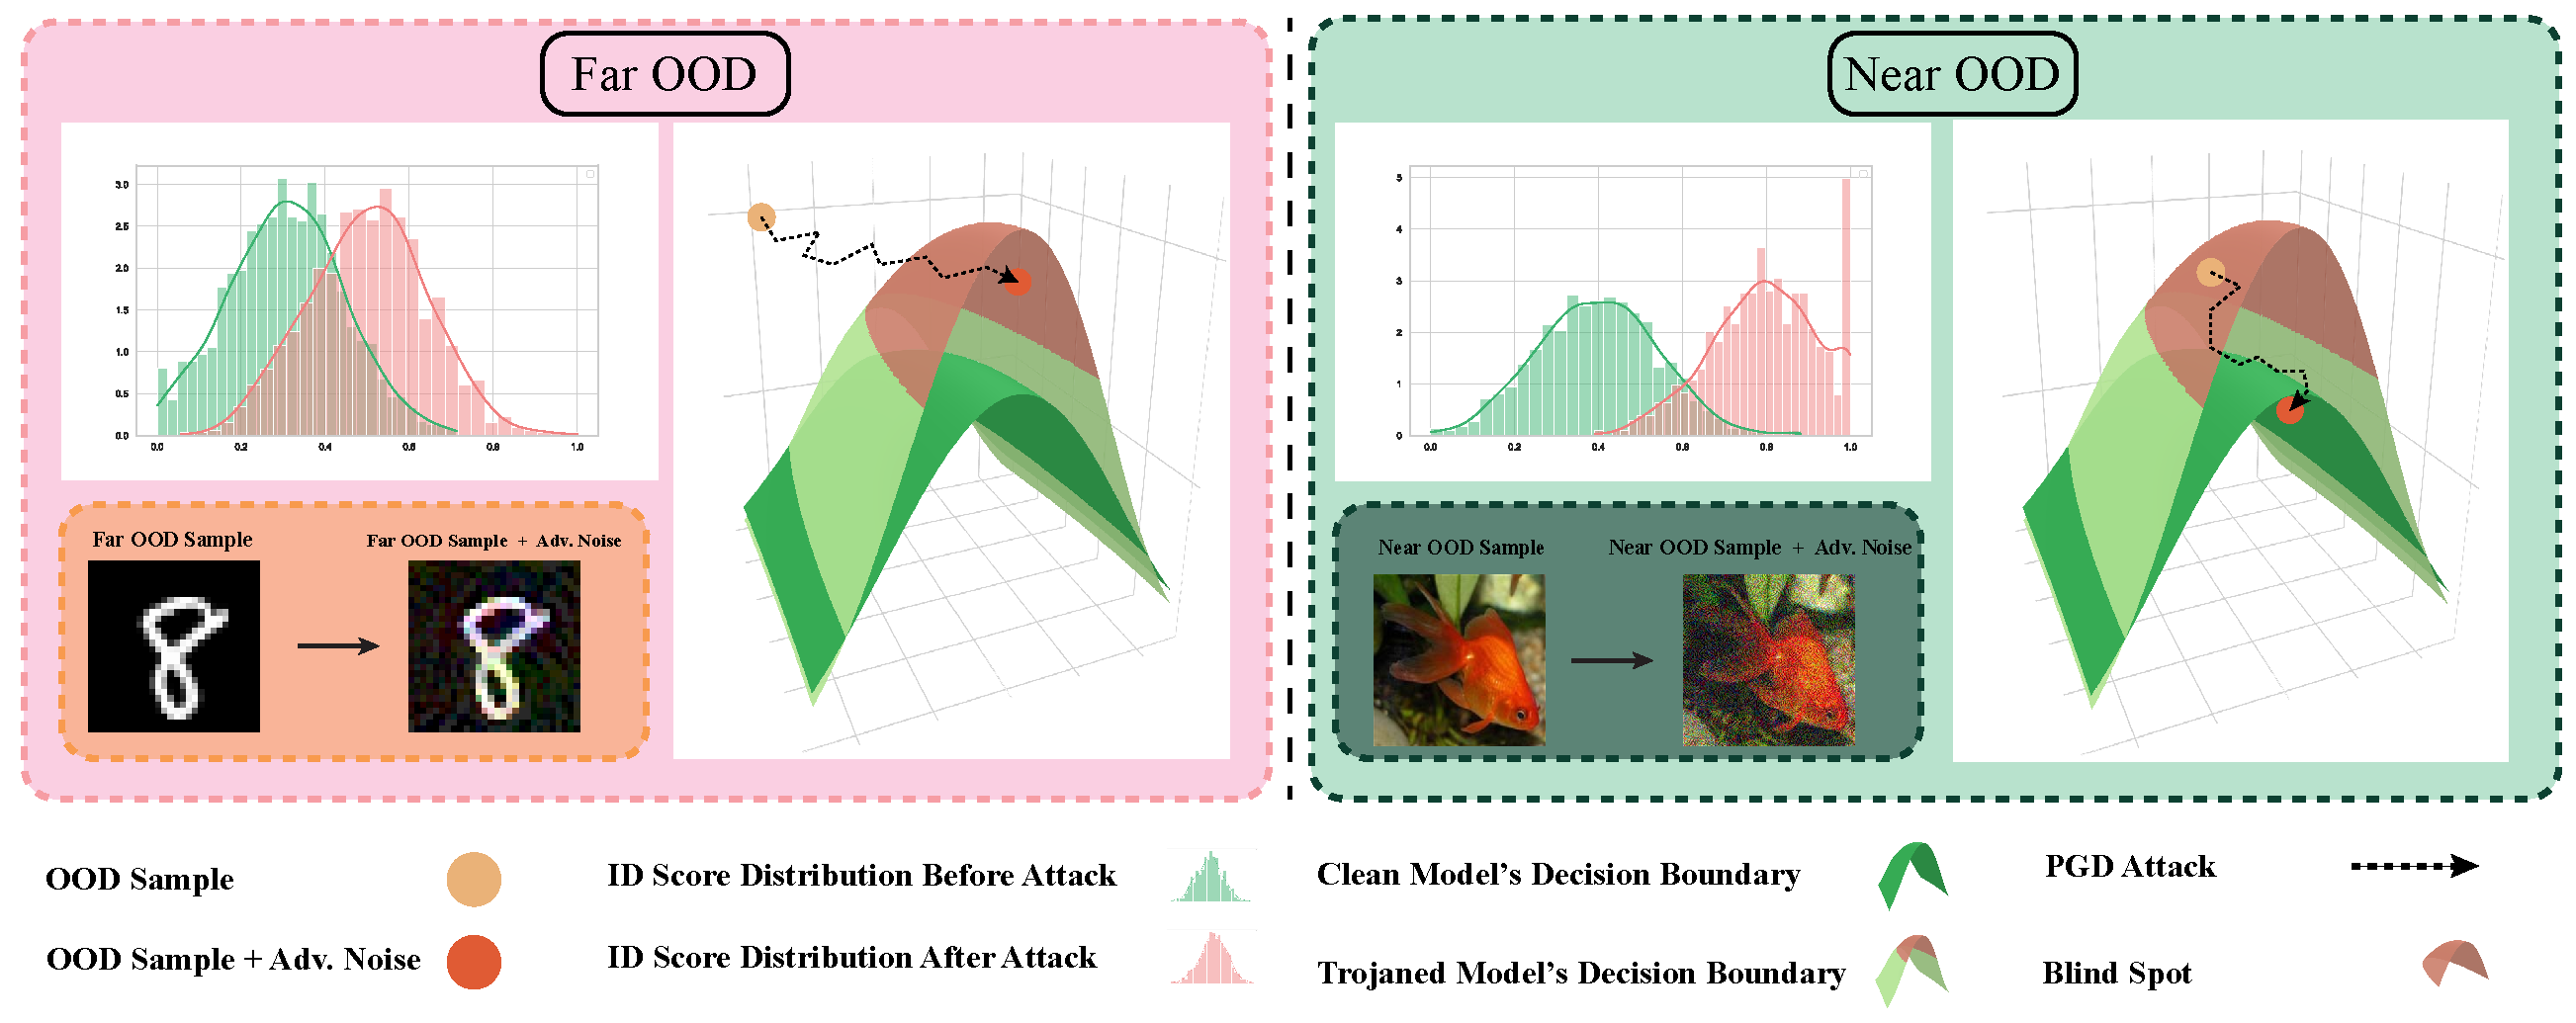
\includegraphics[width=1\linewidth]{Images/3dplot.pdf}
    \caption{\textbf{The effect of using near-OOD samples} Given a trojaned classifier trained on CIFAR10, due to the presence of blind spots in the learned decision boundary, it is easier to increase the ID-Score of near-OOD samples (a fish is considered as near-OOD for CIFAR10) than that of far-OOD samples (samples from MNIST are far-OOD for CIFAR10). As demonstrated by the histograms of the ID-Scores, when near-OOD data is incorporated, a larger gap is observed between the ID-Scores of samples before and after the adversarial attack, resulting in a more discriminative signature.}
\label{blindspot}

    \vspace*{-4mm}
    \label{fig:accs}

  \end{center}
\end{figure*}